



\documentclass[12pt]{article}

%Import packages
\usepackage{amsmath}
\usepackage{listings}
\usepackage[utf8]{inputenc}
\usepackage{algpseudocode}
\usepackage{algorithm}
\usepackage[]{hyperref}
\usepackage{url}
\usepackage{pgfgantt}
\usepackage{comment}
\usepackage{array}
\usepackage[section]{placeins}
\usepackage{array,xstring}
\usepackage{numprint} 
\usepackage{pdflscape} %%landscape
\usepackage{rotating}
\usepackage{graphicx}

\hypersetup{
    pdftitle={Tarea 1 PLN},
    bookmarksnumbered=true,     
    bookmarksopen=true,         
    bookmarksopenlevel=1,       
    colorlinks=true,            
    pdfstartview=Fit,           
    pdfpagemode=UseOutlines,    % this is the option you were lookin for
    pdfpagelayout=TwoPageRight,
    urlcolor=blue,
    linkcolor=blue,
    citecolor=red
}

\title{Tarea 1 \\ IPLN} 
\author{
  Victor Díaz \\
  Valentina Da Silva \\
  Leonardo Clavijo 5.054.830-5
}
\date{\today}


\begin{document}
\maketitle

\begin{abstract}
En este presente documento se procede a la explicación, tanto de la implementación de la aplicación, así como los parámetros de configuración necesarios para la ejecución de la misma \ldots
\end{abstract}

\newpage

\tableofcontents

\newpage

\section{Introduction}
En la presente aplicación se trabajó en base a dos metodologías de procesamiento de datos, mediante el uso de WebServices y una aplicación local(LAN) del servico Freeling.
Por lo tanto en la implementación contamos con dos modos de ejecución, esto puede ser útil para el caso de los usuarios que no cuenta con un servidor Freeling local, pero sí mediante una arquitectura orientada a servicios.
Al pensar en ambos casos, tenemos la ventaja de que si no contamos con alguno de ellos, podemos utilizar el otro método.

\section{Requerimientos}
\subsection{Librerías}\label{lib}
Para la correcta ejecución de la aplicación es necesario contar con el siguiente conjunto de librerías:
\begin{itemize}
  \item suds :  Para utilizar la aplicación mediante Webservices, se trata de una librería que permite la creación de estructuras orientadas a webservices, utilizando el protocolo SOAP.
  \item mathplotlib: Se utiliza para realizar las gráficas pertientes al requerimiento 4.b del laboratorio.
  \item openpyxl : Librería utilizada para la lectura de archivos xls, para el caso en particular el archivo que contiene los comentarios a ser procesados.
\end{itemize}

Los mismas pueden ser agregadas fácilmente utilizando pip o easy-install.
\begin{itemize}
  \item suds : pip install suds-jurko | easy\_install suds-jurko.
  \item mathplotlib : pip install matplotlib | easy\_install -m matplotlib.
  \item openpyxl : pip install openpyxl | easy\_install openpyxl.
\end{itemize}


\subsection{Freeling}\label{free}
Para ejecutar la aplicación utilizando un servidor local, es necesario contar con la aplicación Freeling y ejecutarla en modo servidor, para ello se recurre a la siguiente orden vía línea de comandos:
$analyze$ $-f$ $./config/es.cfg$ $--server$ $--port$ $50005$ $\&$
Donde es.cfg es la configuración general de Freeling para lograr el correcto procesamiento del léxico en cuestión, de esto se tratará en la sección 'Configuraciones Freeling'\ref{configFree}; 50005 es el puerto en el que el servidor escucha los pedidos.
Una vez que se realizó este paso correctamente, podemos ejecutar nuestra aplicación Python. 

\subsubsection{Configuración}\label{configFree}
Los parámetros que se utilizaron para configurar Freeling en modo servidor fueron los siguientes(./config/es.cfg):
\begin{itemize}
\item AffixAnalysis=no : No es necesario en este caso.
\item MultiwordsDetection=yes : Se utiliza para detectar palabras múltiples en una 'string' ya que es habitual errores de tipeo como la falta de espacios o la introducción del caracter $.$ como separador.
\item NumbersDetection=yes : Opcional, se optó por introducirlo aunque aporte en menor proporción.
\item PunctuationDetection=yes : Detecta la puntuación que posteriormente se excluye de las palabras finales.
\item DatesDetection=no : No es necesario en este contexto, puesto que en esta categoría de comentarios no requiere tal precisión para procesar.
\item QuantitiesDetection=no : No es necesario procesar este tipo de magnitudes, se toma como una palabra cualquiera. 
\item DictionarySearch=yes : Para definir el lema, es útil que se encuentre en el diccionario para generar un tag correcto.
\item ProbabilityAssignment=yes : En algún caso podría ser necesario.
\item OrthographicCorrection=no : No sería una idea negativa utilizarlo, aunque para el caso no es una prioridad a tener en cuenta.
\item NERecognition=no : Identificar nombres por ejemplo no aporta calidad a la solución, además se observa comentarios como "Genial, Me Ha Atrapado la película", en realidad genera problemas cuando estamos agrupando las palabras positivas y negativas ya que con esta opción agruparía en un conjunto "Me Ha Atrapado" y se pedería lemas que aportan datos a la solución.
\end{itemize}
Estos fueron las configuraciones más importantes a tener en cuenta en el análisis morfológico, se deja a consideración el archivo ubicado en $./config/es.cfg$ para más detalles, además el mismo debe procesarse cuando se inicia el servicio de Freeling.

\section{Ejecución}
Para ejecutar la aplicación, únicamente se le debe brindar permisos de ejecución al archivo $tarea_1.py$, y mediante línea de comandos la siguiente orden:
$./tarea_1.py$
O $./tarea_1.py -w$ para ejecutarlo utilizando webservices anteriormente descripto.

\section{Visualización}

Se muestra la interacción del sistema, según el modo de ejecución.
\begin{figure}[!h]
  \centering
    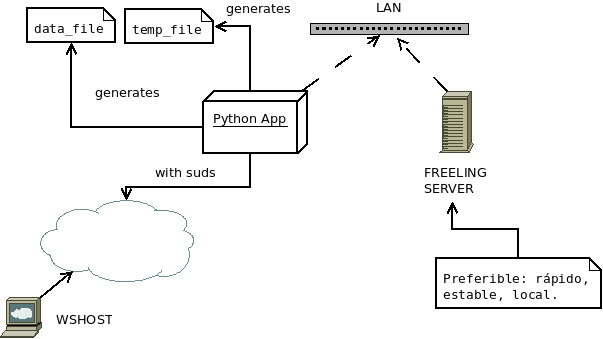
\includegraphics[width=0.8\textwidth]{./fig/arq.png}
  \caption{Interacción}
  \label{fig:arq}
\end{figure} 


\section{Implementación}
Se procede a la descripción de la implementación del programa. Para ello se utilizaron dos clases básicas para las configuraciones:
\begin{enumerate}
   \item Utils : que se encuentra en el mismo archivo a ejecutar $tarea_1.py$, la misma se encarga de realizar operaciones de lectura y escritura en los archivos, así como el porcesamiento de los datos utilizando Freeling.
   \item WebService : la misma se encuentra en el archivo webservices.py, se utiliza para cargar las especificaciones del servicio web en cuestión, además de brindar la implementación de solicitud y procesamiento de del léxico. Básicamente devuelve una lista con todas las palabras con su respectivo tag, lema y probabilidad.
 \end{enumerate} 

A continuación se describe las funciones definidas en el archivo $tarea_1.py$, específicamente de la clase útils.
\subsection{loadXLSFile}
Encabezado: $def$ $loadXLSFile(self)$
Cuando se instancia la clase $Utils$, en sus atributos privados se encuentran ciertos parámetros que definen las condiciones a tener en cuenta para la lectura del archivo $.xlsx$, en particular el nombre del mismo $\_\_comment\_file$ y el rango de las celdas que deben ser procesadas($\_\_xls\_range$), básicamente utiliza la librería descripta en la sección anterior librería \ref{lib}, y devuelve como resultado el rango de celdas especificado por el parámetro en cuestión, el cual será iterado en la función main.

\subsection{loadStopwords}
Encabezado: $def$ $loadStopwords(self)$
En este caso se carga en un diccionario las palabras vacías que se suministran en el archivo $stopwords.txt$, se devuelve un diccionario para el rápido procesamiento posterior llevado a cabo.


\subsection{loadSubjetiveElems}
Encabezado: $def$ $loadSubjetiveElems(self)$
Esta función carga el léxico proporcionado en el archivo $listaElementosSubjetivos.pl$, devolviendo un diccionario como estructura para su posterior procesamiento.


\subsection{lematization\_freeling\_client}
Encabezado: $def$ $lematization\_freeling\_client(self, comment, stopwords)$.
Argumentos:
\begin{itemize}
  \item $comment$ : Comentario particular a ser procesado.
  \item $stopwords$ : Se trata de un diccionario con las palabras vacías a ser excluídas en nuestro procesamiento.
\end{itemize}
Su funcionalidad principal es tomar un comentario específico mediante una string, guardarlo en un archivo particular llamado $temp_file$, para invocar la orden que se encargará de enviarle los datos al servidor local Freeling. Posterior a dicho procedimiento, se procede a la lectura del archivo de salida que genera el servidor, el mismo se encuentra en el archivo temporal $data_file$, de esta forma se lee completamente el archivo y se extra el tag, lema y probabilidad de todas las palabras presentes en el comentario.
Se utiliza como función para garantizar la legibilidad de la función principal $main$.


\subsection{plot}
Encabezado: $def$ $plot(self, listaPlot, n\_groups, filename)$ \\
Argumentos:
\begin{itemize}
  \item listaPlot : Contiene una lista ordenada con la siguiente tupla de datos $(Palabra, Comentarios)$, donde $Palabra$ es el lema a graficar, y $Comentario$ es la cantidad de veces comentarios en la que $Palabra$ está presente. Notar que se contabiliza únicamente una vez la palabra por comentario, para evitar casos extremos que degraden el comportamiento del programa en cuestión, ej. Comentario = "Hola, hola, hola, ...", si se evalúa globalmente, puede perjudicar el estudio en cuestión.
  \item n\_groups : Cantidad de palabras que serán procesadas en la salida gráfica.
  \item filename : Nombre del archivo de salida del procesamiento gráfico, la imagen será guardada en el directorio $figures$ localizado en la ruta donde se procesa la aplicación.
\end{itemize}

Su funcionalidad lo describe el nombre de la función, retorna una salida gráfica mediante archivos $.png$ con los resultados obtenidos.
En la implementación en cuestión se invoca cinco veces la presente función, generando los archivos a continuación:
\begin{itemize}
  \item AllWords.png : Se encuentran las $n\_groups$ palabras ordenadas de forma decreciente, en este caso no se distingue entre palabras positivas y negativas, básicamente es un conteo global de todas las palabras procesadas.
  \item NegativeSubjetive.png : En este caso se suministra el top $n\_groups$ palabras presentes en comentarios con un a puntuación 1 o 2 intersección palabras negativas suministradas en el archivo $listaElementosSubjetivos.pl$.
  \item PositiveSubjetive : Análogo al caso anterior pero aplicado a palabras positivas.
  \item NegativeWords.png : Ilustra las palabras presentes en los comentarios con evaluación negativa(1 y 2).
  \item PositiveWords.png : Análogo caso anterior pero teniendo en cuenta palabras con evaluación positiva.
\end{itemize}


\subsection{main}
Este bloque se encarga de tomar las funciones anteriormente mencionadas y procesar el algoritmo de forma adecuada.
Se presenta a continuación un pseudo-código de la implementación.

\begin{algorithmic}
  \State $xls \gets cargar\_comentarios()$
  \State $stopwords \gets cargar\_palabras\_vacias$
  \State $subjetivas \gets cargar\_palabras\_subjetivas$
  
  \For{$comentario$ in $xls$}
    \State {$lista \gets lematizar(comentario)$}
     \For{$palabra$ in $lista$}
       \State {$(pos, neg) \gets agregarDiccionario()$}      
     \EndFor
  \EndFor
  
  \State $imagenes \gets graficarResultados(pos, neg)$
\end{algorithmic}

La simplicidad que brinda Python para el procesamiento de datos, básicamente resume el pseudocódigo en la implementación en sí misma, salvo detalles menores que requieren un procesamiento refinado.


\section{Eficiencia}
La complejidad del un programa se reduce a las estructuras utilizadas, la correcta utilización de las mismas implica implica impacto directo sobre la eficiencia del programa. Para ello se utilizaron Diccionarios para almacenar las palabras contenidas en los comentarios, de esta forma poder acceder en orden 1. La búsqueda se reduce a investigar si la llave(key) de indexado se encuentra presente en el Diccionario. Por lo contrario, utilizando listas, la performance al procesar una lista mayor de comentarios tiene un impacto negativo en tiempos de ejecución.
Se recomienda fuertemente utilizar el modo de ejecución con servidor local con Freeling, de esta forma se reducen costos de tráfico de red y posibles "errores de ejecución" ajenas al programa diseñado.
La simplicidad de utilizar expresiones regulares para realizar reemplazos y búsquedas impacta positivamente en el desempeño del programa, es por ello que se utilizaron las mismas para sintetizar la lista de elementos subjetivos. Además agrega elegancia a la solución.

La captura de excepciones permite brindarle al usuario un detalle sobre los requerimientos que debe satisfacer para ejecutar correctamente el programa, para ello se implementó un manejo de las mismas en los casos de lectura y escritura de archivos así como también en el caso del WebService, que en ocasiones adversas no responde de forma adecuada.

\section{Conclusiones}\label{conclusions}
\subsection{Implementación}
Lenguaje de programación alto nivel, presenta gran diversidad de librerías internas como externas que facilitan la tarea en gran parte. Su alto nivel permite no definir tipos específicos y de esta forma se trabaja de manera más fluida, aunque esto pueda llegar a confusiones si no se declaran correctamente las variables con un nombre adecuado.
Escaso tiempo de implementación, dada la versatilidad, el tiempo de implementación se reduce considerablemente considerando con otros lenguajes de programación.
Al ser lenguaje interpretado, es sencillo de utilizarlo para realizar tareas de menor porte que requieran una cantidad de datos moderado. Se desconoce funcionamiento con gran cantidad de comentarios(potencialmente superior a el caso propuesto).
Codificación legible, si se utilizan estándares como el propuesto en la implementación(PEP8), brinda a terceros la posibilidad de tener un código legible y simple a la lectura.
Portabilidad con sistemas operativos no es 100\% satisfactorio, para desarrollar existieron problemas específicamente de codificación de las palabras, en entornos UNIX no existe dicho problema, mientras que en sistemas Windows existieron los problemas mencionados, además de todo el proceso de instalación del lenguaje(tedioso en Windows) así como también las herramientas(Freeling).
Salvo detalles menores es un lenguaje adecuado para utilizarlo para el procesamiento de datos a pequeña y mediana escala.
Al brindar características de un paradigma funcional(map, zip, etc), brinda simplicidad y 'ahorro' en cantidad de líneas utilizadas en total.
La unificación derivada de la programación lógica, combinada con paradigma funcional hace un lenguaje poderoso con lo que refiere manipulación de datos en general, una característica deseable también como  ser la posibilidad de generar APIs con swig y combinar la eficiencia de c++ en la ejecución de algoritmos que requieran uso excesivo del recurso CPU. 

%\bibliographystyle{abbrv}
%\bibliography{simple}

\end{document}
